\let\accentvec\vec
\documentclass[fleqn]{llncs}
\let\spvec\vec
\let\vec\accentvec

% make a proper TOC despite llncs
\setcounter{tocdepth}{2}
\makeatletter
\renewcommand*\l@author[2]{}
\renewcommand*\l@title[2]{}
\makeatletter

\usepackage[utf8]{inputenc}%cesar
\usepackage{multirow}
\usepackage{epsfig}
\newcommand{\todo}[1]{\fbox{\sc To do: #1}}
\newcommand{\sidenote}{\marginpar{$\star$}\small\bf}
\newcommand{\ra}{\rightarrow}
\def\C{\cal C} %Cesar
\def\F{\cal F}
\def\T{\cal T}

\long\def\comment#1{}

\usepackage{amssymb}
\usepackage{amsmath}%para el cases

\usepackage{yhmath} % \widetriangle
\usepackage{tipa}   % many
\usepackage{phonetic}  % \textipa and related symbols
\usepackage{extraipa}  % \subdoublevert
\usepackage{mathabx} % \widecheck  % THIS IS NOT STANDARD. NEEDS TO BE MANUALLY INSTALLED.
\usepackage{stmaryrd} % \Ydown
\usepackage{harpoon} % \overleftharpdown, \overleftharp
\usepackage{mathtools} % \overbracket
\usepackage{accents}  % fabrication of new accents (\accentset, \underaccent)
% The accents package facilitates the fabrication of accents in math mode. Its \accentset command enables
% any character to be used as an accent. For instance, \accentset{\star}{f} produces \ ?
% f " and
% \accentset{e}{X} produces \ e
% X". \underaccent does the same thing, but places the accent beneath the
% character. This enables constructs like \underaccent{\tilde}{V}, which produces \
% accents provides
% other accent-related features as well; see the documentation for more information.

% New command. Cross below the letter.
\newcommand{\textsubcross}[1]{\tipaloweraccent{24}{#1}}

% SHORTCUTS

% Annotated
\newcommand{\annl}[1]{\textopencorner{#1}}   %{$\llcorner{}{\mbox{#1}}$}
\newcommand{\annr}[1]{\textcorner{#1}}   %{$\lrcorner{}{\mbox{#1}}$}

% Non-annotated
\newcommand{\nonl}[1]{$\llcorner{}{\mbox{#1}}$}   %{\textopencorner{#1}}
\newcommand{\nonr}[1]{$\lrcorner{}{\mbox{#1}}$}   %{\textcorner{#1}}


% Silent, stress and separators (beneath)  
% Hint: all start with 's'
\newcommand{\si}[1]{\textsubcross{#1}}
\newcommand{\st}[1]{\textsyllabic{#1}}
\newcommand{\stst}[1]{\subdoublevert{#1}}
\newcommand{\se}[1]{\textraising{#1}}
\newcommand{\sel}[1]{\textadvancing{#1}}
\newcommand{\ser}[1]{\textretracting{#1}}
\newcommand{\selr}[1]{\sel{}\textsubplus{}}
\newcommand{\serl}[1]{\textsubplus{}\ser{}}

% Consonants (beneath)
% Hint: all end with 'o'
\newcommand{\co}[1]{\textsubring{#1}}
\newcommand{\io}[1]{\d{#1}}
\newcommand{\vo}[1]{\textsubwedge{#1}}
\newcommand{\no}[1]{\textsubcircum{#1}}

\newcommand{\svo}[1]{\textinvsubbridge{#1}}
\newcommand{\sno}[1]{\textsubbridge{#1}}

\newcommand{\hvo}[1]{\b{\textinvsubbridge{#1}}}
\newcommand{\hno}[1]{\b{\textsubbridge{#1}}}

\newcommand{\w}[1]{\textsubw{#1}}
\newcommand{\y}[1]{$\underaccent{\Ydown}{\mbox{#1}}$}

% Vowel Introductions
\newcommand{\uu}[1]{$\breve{\mbox{#1}}$}
%\newcommand{\ii}[1]{\.{#1}}
\newcommand{\ii}[1]{$\dot{\mbox{#1}}$}
\newcommand{\ai}[1]{\textcircumdot{#1}}
% schwa symbol
\newcommand{\sch}[1]{$\accentset{\backepsilon}{\mbox{#1\upbar{}}}$}  % package textcomp
\newcommand{\ssch}[1]{$\accentset{\backepsilon}{\mbox{#1}}$}  % package textcomp
%\, a thin space
%\! a negative thin space

% Vowels (above)
% Hint: all three letters
\newcommand{\pln}[1]{\textvbaraccent{#1}}
\newcommand{\ppln}[1]{\textvbaraccent{#1}}
\newcommand{\nat}[1]{\~{#1}}
\newcommand{\nnat}[1]{$\widetilde{\mbox{#1}}$}
\newcommand{\brd}[1]{\={#1}}
\newcommand{\bbrd}[1]{$\overline{\mbox{#1}}$}
\newcommand{\rnd}[1]{\r{#1}}
\newcommand{\rrnd}[1]{\r{#1}}
\newcommand{\clr}[1]{\^{#1}}
\newcommand{\cclr}[1]{$\widehat{\mbox{#1}}$}
\newcommand{\opq}[1]{\v{#1}}
\newcommand{\oopq}[1]{$\widecheck{\mbox{#1}}$}
\newcommand{\dip}[1]{$\widetriangle{\mbox{#1}}$}  % Problems
\newcommand{\ddip}[1]{$\widetriangle{\mbox{#1}}$}
\newcommand{\idp}[1]{\`{#1}}
\newcommand{\iidp}[1]{$\overleftharpdown{\mbox{#1}}$}
\newcommand{\udp}[1]{\'{#1}}
\newcommand{\uudp}[1]{$\overleftharp{\mbox{#1}}$}
\newcommand{\iot}[1]{\.{#1}}
\newcommand{\cnt}[1]{\"{#1}}
\newcommand{\ccnt}[1]{\"{#1}}
\newcommand{\red}[1]{\crtilde{#1}}
\newcommand{\rred}[1]{\crtilde{#1}}


% Useful to group more than two letters, before applying the annotation.
\newcommand{\group}[1]{\underline{#1}}
% Other options: \svo{\underline{ssi}},  {\svo{$\undergroup{ssi}$}}, {\svo{$\underleftrightarrow{ssi}$}}, {\svo{$\underlinesegment{ssi}$}}


%Stuff I use

\usepackage[backend=bibtex,style=numeric,sorting=none]{biblatex}
\bibliography{Refs.bib}
\usepackage[left=2.5cm,right=2.5cm,top=2.5cm,bottom=2.5cm]{geometry}
\pagestyle{plain}

\begin{document}
\begin{titlepage}

\title{Project Specification: Annotated English}
\author{KJ Tsanaktsidis}
\institute{FIT3036, Monash University}
\maketitle
\thispagestyle{empty}

\abstract{`Annot\st{a}t\iot{e}d \iot{E}nglish' is a proposal for clarifying the pronunciation of English words by defining unambiguous rules and adding diacritics representing exceptions to these rules. This is useful for people who can read English, but have difficulty with pronunciation. This proposal describes a tool for deducing the phonetic IPA transcription of an Annotated English word. The functionality of the tool is defined, and a high-level overview of the proposed software architecture is given. A project plan and a test plan outline how the project is to be delivered. It is hoped that the development of this tool will help with the adoption of Annotated English and prove useful to English readers looking to correct their pronunciation.}

\vspace{10mm}
\textbf{Word count:} 1868 words

\end{titlepage}

\tableofcontents
\thispagestyle{plain}

\newpage

\section{Introduction}
The English language has a truly horrid system of spelling compared with almost every other European language. Often, the way a word is written down has very little bearing on how a word is actually pronounced. The situation is especially bad for vowels \cite{bellspell}. This makes it difficult for people who may read English proficiently to actually speak it well.

Various proposals have been developed to reform the spelling of the English language to make words more closely indicate their pronunciation (for example, Interspell \cite{interspell}). However, schemes such as this have a fundamental problem in that they require extensive retraining of generations of both native and non-native English speakers to stick.

Annotated English \cite{jose} is a system developed by Jos{\'e} Hern{\'a}ndez-Orallo to indicate the pronunciation of English words without changing their spelling. This is achieved by defining a set of unambiguous rules governing the pronunciation of English words. A set of diacritic symbols is also defined which can change the sound that letters would otherwise make. For example, in this scheme, the words `Annotated English' would be written as `Annot\st{a}t\iot{e}d \iot{E}nglish'. Appendix B of \cite{jose} describes a set of {\LaTeX} commands which can render the required annotations. Using these commands, the text `\texttt{Annot{\textbackslash}st\{a\}t{\textbackslash}iot\{e\}d {\textbackslash}iot\{E\}nglish}' produces the correct annotated output.

The advantage of this system is that the spelling of the text is not touched. A proficient English speaker can completely ignore all of the annotations and read normally. However, if a reader requires clarification on how a word should be pronounced, they can consult the annotations. Software which processes English text can also filter out the annotations and work as normal.

The pronunciation is deduced by working through 10 stages of processing outlined in \cite{jose}, which gradually transform annotated text into IPA phonemes. IPA is a representation of a word's pronunciation using special symbols where each such symbol represents a single sound. Although several similar representations are possible for the same word \cite{ipapron}, a given IPA string to a very good approximation has only one possible pronunciation. For example, the IPA representation of `Annot\st{a}t\iot{e}d \iot{E}nglish' is `\textipa{"{\ae}n@""teId "I{\:n}glIS}'.

In order for Annotated English to be widely adopted, two pieces of software must exist. First, an encoder program needs to be available which takes as input a text and a pronunciation corpus (perhaps as described in \cite{ipapron}) and produces as output an annotated text. Secondly, a piece of software must exist which reproduces the IPA transcription of an annotated text, so as to assist a reader if required. In this project, we focus on building the latter.

\section{Project Plan}

\subsection{Requirements}
In this project, we wish to build a program which takes an annotated text as input and from this deduces the correct pronunciation of each word. The input will be read in the {\LaTeX} source form outlined in the introduction and in \cite{jose}. This form will need to be parsed and then the sequence of rules outlined in \cite{jose} applied.

The program should then output the IPA representation of the words in the text. This should then be converted into X-SAMPA, a transcription of IPA using only 7-bit ASCII characters \cite{sampa}. From X-SAMPA, it can be fed into a text-to-speech program to verify that the word sounds as it should.

\subsection{Target Platform}
Linux is the target platform for this project. No desktop environment is being targeted; instead, a command-line application will be built. Linux is appropriate for this project because of the first-class availability of an excellent finite-state transducer toolkit FOMA \cite{foma} as well as an X-SAMPA capable text-to-speech engine Pico \cite{pico}. Furthermore, a text-mode application is much simpler to build, and the typical Linux command-line environment is significantly richer in functionality than the Windows equivalent. 

FOMA is a toolkit for producing text-processing applications. The programmer must produce a file containing replacement rules using regular expressions. At build time, the FOMA program compiles these rules into a representation of a finite-state transducer. This is an automata that uniquely specifies output text for every valid piece of input text in an alphabet \cite{fst}. This allows the construction of an Annotated English interpreter by specifying and composing the individual rules as regular expressions.

The application itself will be coded in C. This choice has been made due to the availability of C-language interfaces to both FOMA and Pico, and the relative simplicity of the language.

There are no specific hardware requirements for this application, except that it must be able to run Linux. All testing will be performed on an x86 Intel `Sandy Bridge' machine.

\subsection{Risk Analysis}
One of the greatest risks to this project is that the initial technology choices made may be unsuitable. Should this come to light in the midst of the implementation phase, it is likely that significant amounts of code will need to be rewritten to suit the new language or libraries chosen. This will obviously consume precious time in research and coding.

Discovering unexpected complexity in the Annotated English implementation is also a significant risk to this project. If part way through the implementation of the ruleset a serious problem is encountered, it may be necessary to rework significant parts of the application to change the approach taken. Again, this will likely result in lost time and a failure to meet the deadline.

Significant work has already been undertaken to mitigate these risks through so-called Spike Testing \cite{agile}. This involves producing throw-away code to verify that the concepts and technologies have been understood and work as intended. In this case, a number of the Annotated English rules have already been implemented with FOMA and tested against some of the examples in \cite{jose}. As a result of this work, we have a much better understanding of how to use FOMA, its features, and its limitations. Additionally, several problems with a naive implementation of Annotated English have been identified and solutions developed. Some of these discoveries have informed the high-level design of the application, outlined in the next section.

An additional test has also been performed on the capabilities of the Pico TTS engine. How exactly to make Pico speak out X-SAMPA phonemes has now been identified and verified, and the quality of the output sound has been assessed. This testing has directly informed the choice of Pico as the TTS platform being targeted.

Additional risk mitigation has been undertaken by emailing Dr. Hern{\'a}ndez-Orallo to open a line of communication with him. Already, this has helped resolve one ambiguity and provide some useful advice on how to proceed. This channel might be used to gain assistance during the project should more seemingly intractable issues arise.

\subsection{Project Schedule}
The application must be ready for demonstration by Tuesday the 20th of April \cite{unitguide}. This gives about 6 weeks starting from the 8th of April. In this time, all development and testing of the project must be conducted.

Dr Hern{\'a}ndez-Orallo has indicated \cite{email} that he expects the Annotated English rules in \cite{jose} to require some tweaking due to unintended conflicts. This suggests that an iterative development approach should be undertaken. A first version of the software will be produced as quickly as possible, preferably within the first three weeks. This will allow ample time for a testing loop, the details of which will be outlined later in the Test Plan section. Rules with unintended side effects can be identified by the output of incorrect pronunciation from the tool; they can then be appropriately narrowed. The cycle of testing then continues until no obvious problems are found. This is illustrated in figure \ref{fig:devflow}.

\begin{figure}[htp]
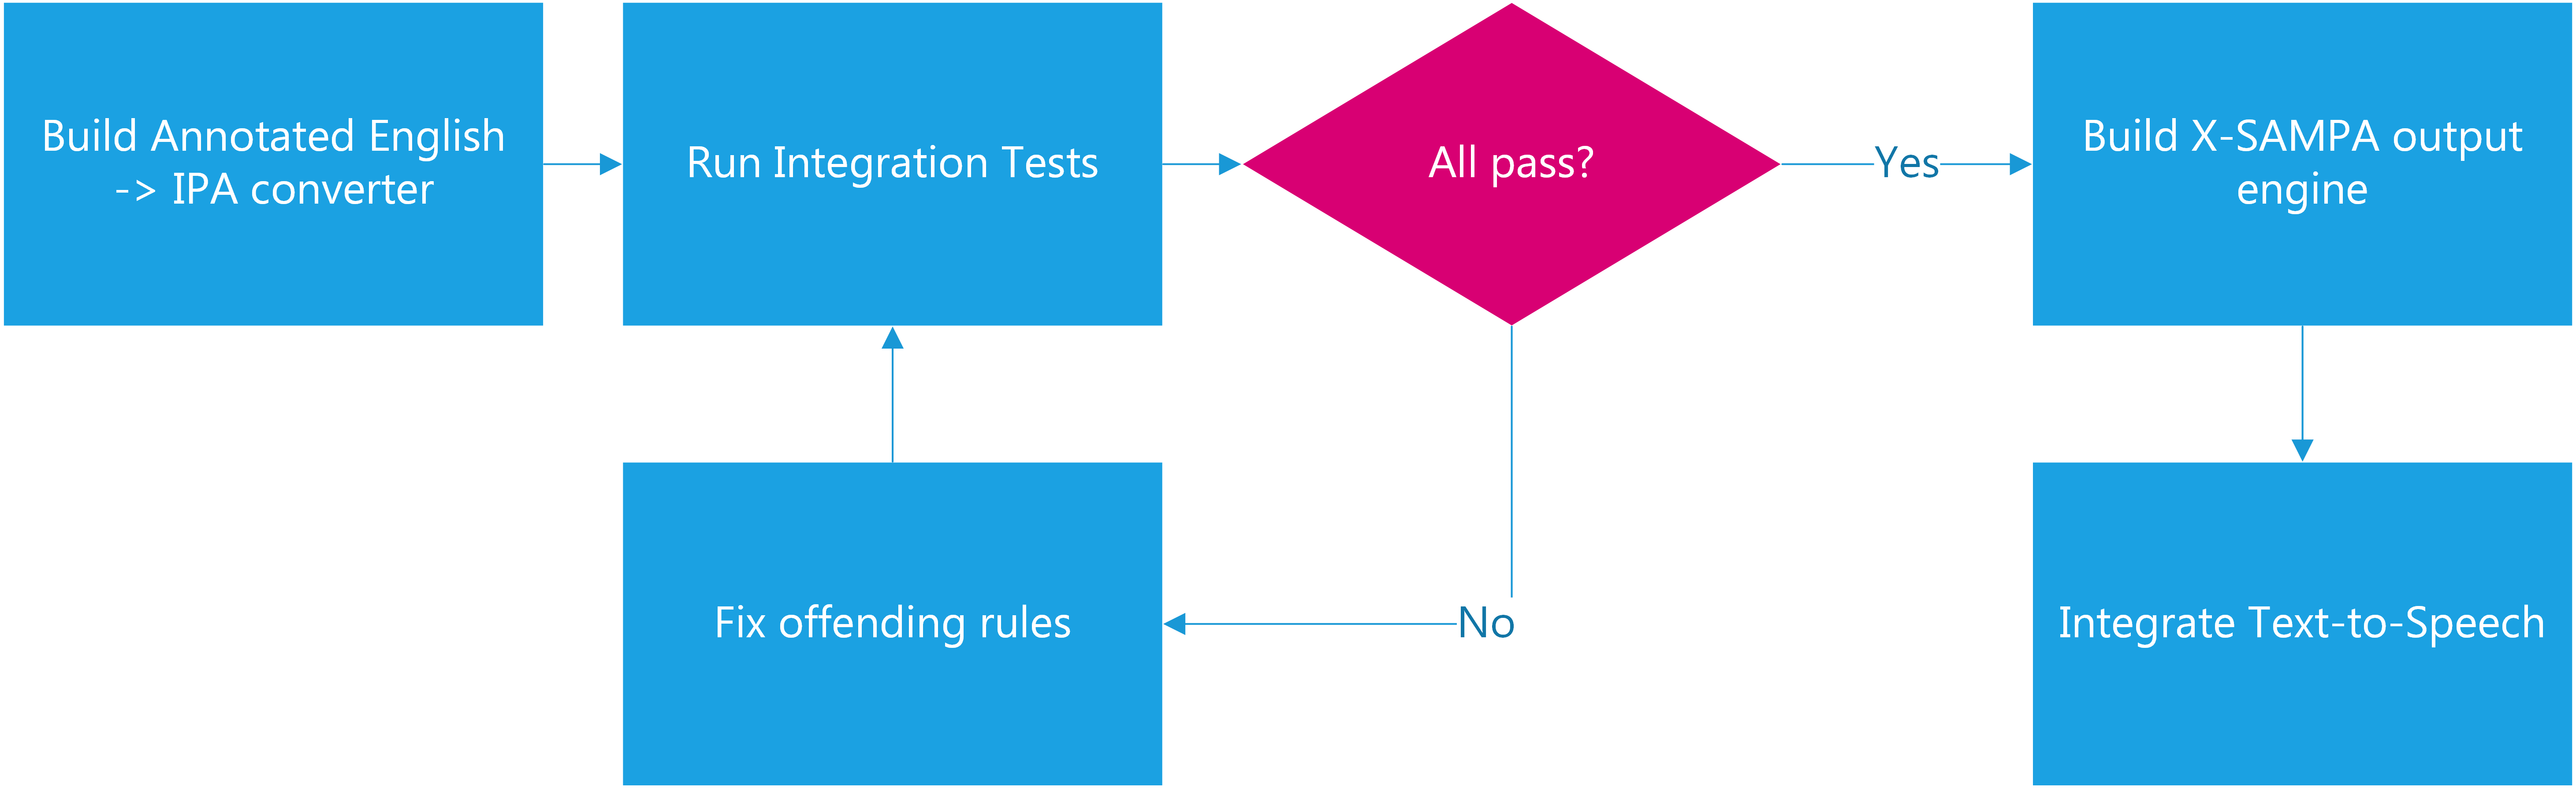
\includegraphics[width=0.9\linewidth]{development_flow.png}
\caption{Flowchart of the proposed development and testing methodology}
\label{fig:devflow}
\end{figure}

The most important aspect of the project is the Annotated English $ \rightarrow $ IPA converter. This aspect will be prioritised in development, so that should it not be possible to implement other features such as TTS in the time allowed, a functional tool is still developed.

\section{Software Design}

\subsection{Software Interface}
As previously noted, the application to be built will have a command-line interface. Annotated English in {\LaTeX} form will be read from standard input. Since all Linux shells will allow the contents of a file to be piped to a program's standard input through input redirection, reading from a file does not need to be explicitly coded. 

Whether IPA or X-SAMPA output is produced will depend on the value of a command-line argument to the program. This output will be written to standard output, where it can be written to a file via output redirection. An additional command-line switch will determine whether or not the TTS engine is invoked to pronounce this output.

\subsection{Processing Pipeline}
The software to be developed in this project is best modeled as a pipeline with several stages. Annotated English input is transformed to IPA by the sequential application of 10 rulesets in \cite{jose} by a transducer, then to X-SAMPA by a 1:1 transliteration process, and finally to speech sounds by the Pico TTS library. However, early testing has uncovered the need for a pre-processing stage before the finite-state transducer.

In some circumstances, Annotated English allows the nesting of {\LaTeX} commands to place multiple annotations on a letter- for example, an accented letter can have a stress as in \pln{a}nth\st{\pln{o}}logy (\texttt{{\textbackslash}pln\{a\}nth{\textbackslash}st\{{\textbackslash}pln\{o\}\}logy}). In a regular expression engine such as FOMA, it is impossible to detect whether or not something is in such a set of nested \{\} brackets. Matching brackets is the classic non-regular, context-free grammar \cite{fst}.

A pre-processing step will be included to deal with such cases of nested annotations. This will principally consist of a pushdown automaton, a computational model capable of dealing with context-free grammars \cite{theoryofc}. The \texttt{{\textbackslash}group} command is purely a visual aid and can be removed altogether, whilst nested stresses can be replaced with special tokens.

The various steps in the pipeline will be wired together with the C-language API's of FOMA and Pico. The entire pipeline is illustrated visually in figure \ref{fig:progpipe}.

\begin{figure}[htp]
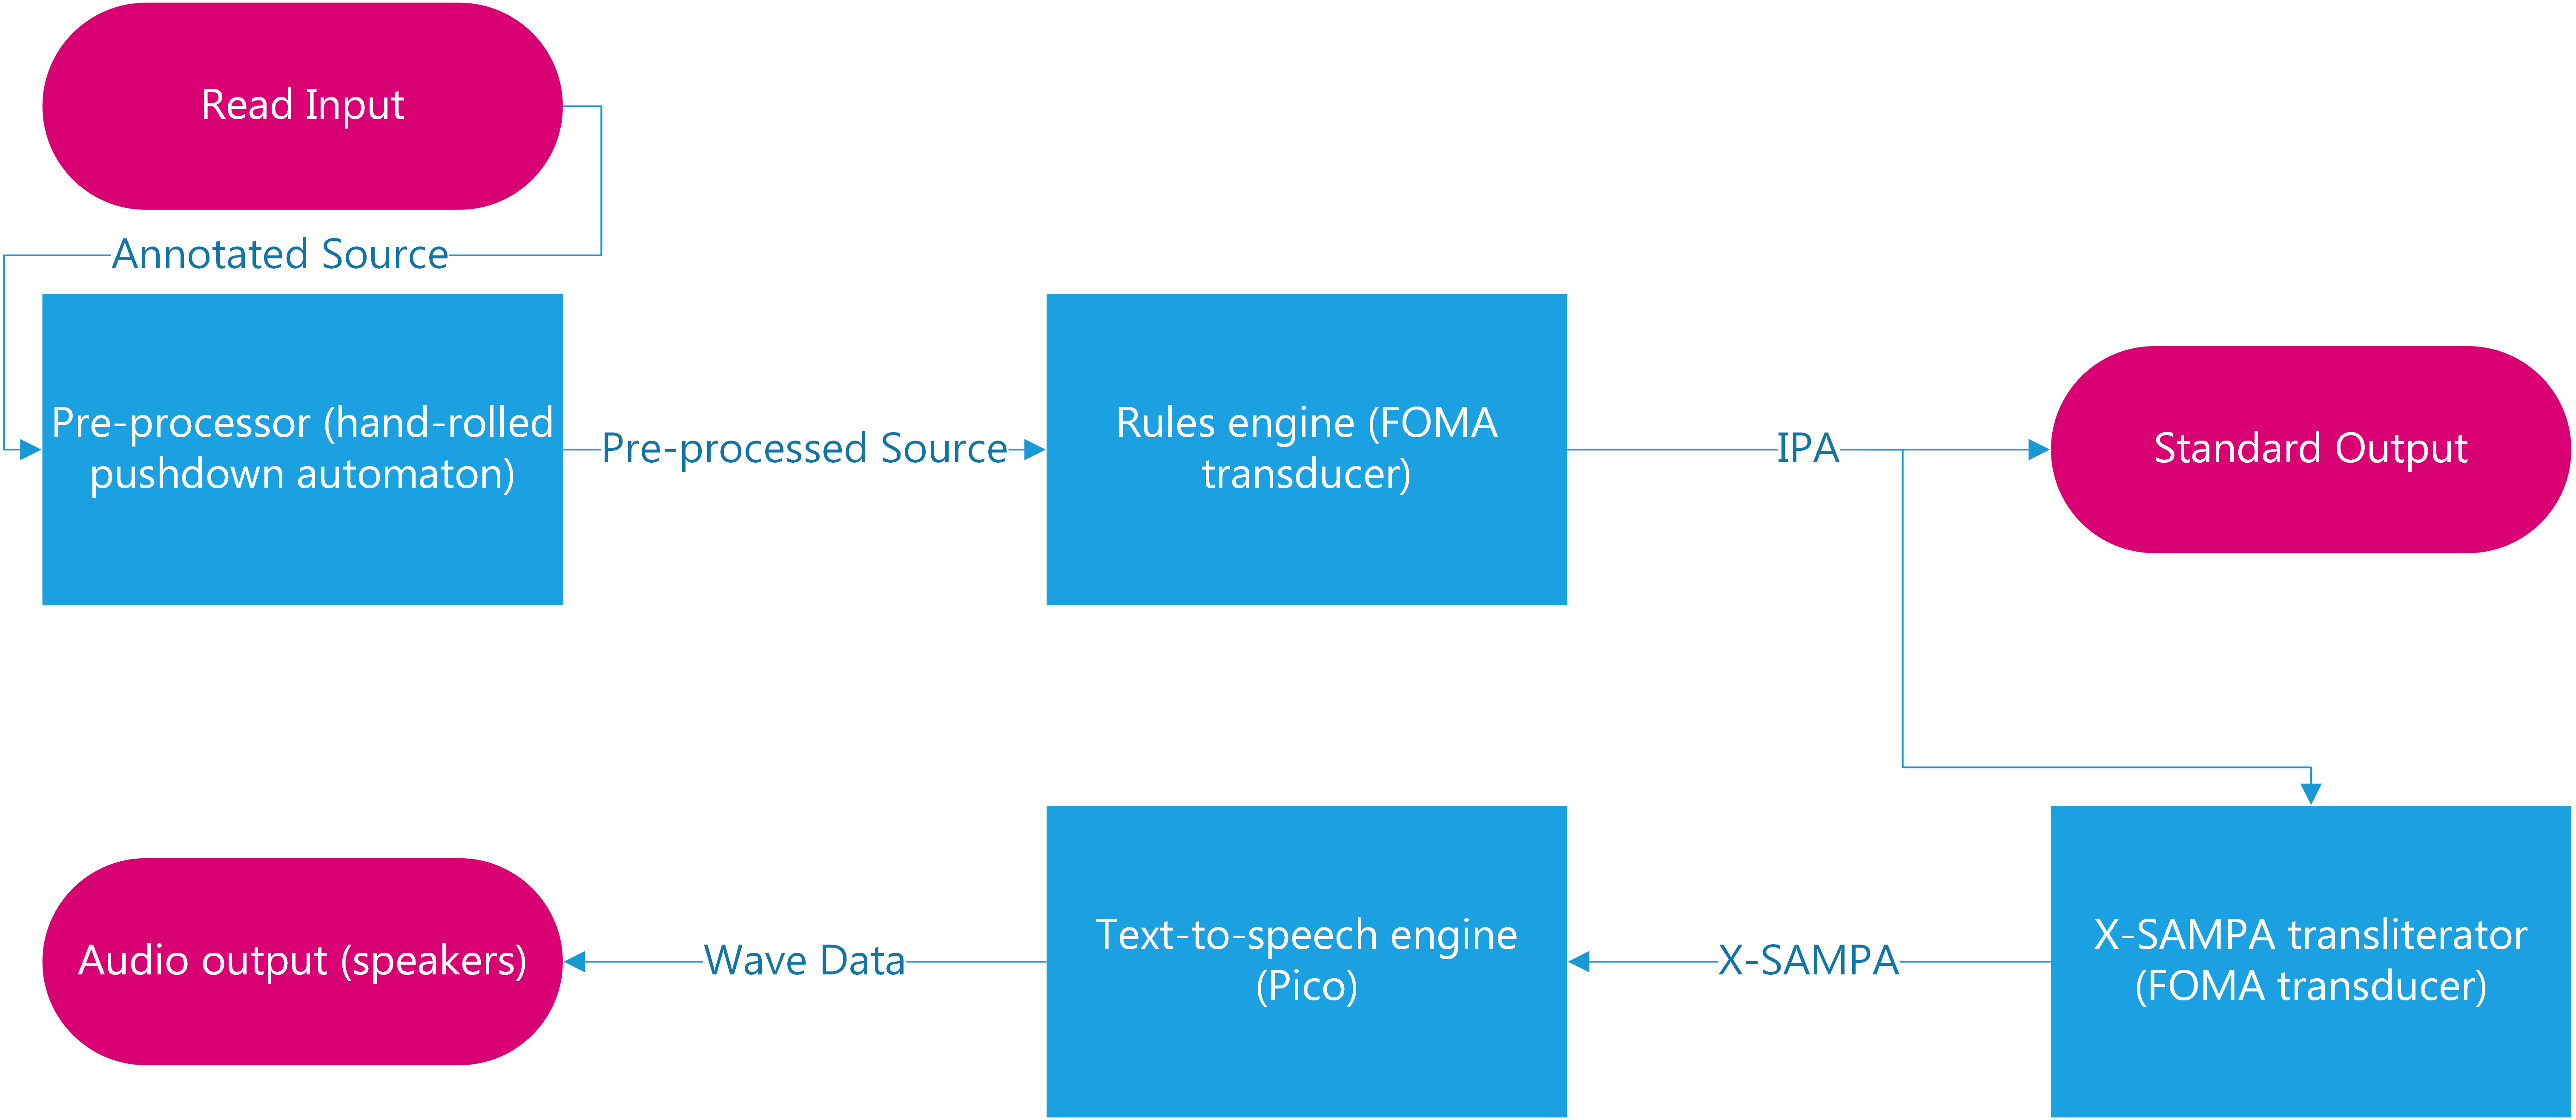
\includegraphics[width=0.9\linewidth]{data_flow.png}
\caption{Planned data flow in the software. The pre-processing step is implemented with a pushdown automaton, whilst the other text processing steps are implemented as FOMA transducers}
\label{fig:progpipe}
\end{figure}

\subsection{Performance}
Because of the prototype nature of this software, performance is not an especially relevant issue for this project. That said, it is expected that the running time of the software will be linear in the size of the input text. This is because the language accepted by FOMA transducers is strictly regular, and such regular languages can be parsed in \texttt{O(N)} time \cite{theoryofc}.

\section{Test Plan}
As previously mentioned, it is anticipated that the rules in \cite{jose} will need to be modified somewhat in response to their unintended side-effects. It is therefore more likely that the rules themselves will need to change than that they are implemented incorrectly. Under these circumstances, unit testing is of limited usefulness.

Instead, this project will feature a focus on end-to-end integration tests. The Annotated English publication contains a large number of example annotated words. A cross-section of these will be chosen and their IPA pronunciations looked up in a corpus such as that from the Oxford English Dictionary \cite{dico}. These values can then be compared in an automated manner with the output from the program, and inconsistencies debugged.

Once these tests are passing, a manual, auditory test of the TTS output of the software will be conducted. This will verify that the annotated words sound as they should.

\section{Conclusion}
In this document, a program for deducing Annotated English \cite{jose} pronunciations has been described. The high-level design for the system has been outlined, as well as a test plan and a project plan. The risk mitigation steps already taken put the project on the right track for success.

\printbibliography

\vspace{10mm}

\textbf{Word count:} 1868 words
\end{document}
